\section{Experimental Evaluation}
\subsection{Experimental Setup}
For our experiments, we utilized a 12-node cluster, each running Linux (kernel version 3.10) and Apache Spark 2.4. Each node was equipped with 8 cores, providing a total of 96 cores across the cluster. Each core operated with an Intel Xeon CPU at 1.70 GHz, and each node had 4 GB of main memory.

To evaluate the different approaches, we generated three synthetic datasets with varying characteristics, as detailed in Table \ref{tab:datasets}. These datasets were created using the SUMO simulator \cite{krajzewicz_recent_2012}, by importing traffic networks of Berlin and Los Angeles from OpenStreetMap \cite{haklay2008openstreetmap}. We configured SUMO for pedestrian traffic and generated datasets of 10K, 25K, and 50K pedestrian trajectories. The total duration of the trajectories was set to 10, 30, and 60 minutes, respectively, with positions of pedestrians recorded at one-minute intervals.

\begin{table}
    \centering
    \caption{Description of datasets.}\label{tab:datasets}
    \begin{tabular}{cccc}
        \hline
        Dataset & Number of Trajectories & Total number of points & Maximum Duration (min) \\
        \hline
         Berlin10K &  10000 & 97526 & 10\\ 
         LA25K &  25000 & 1495637 & 30\\
         LA50K &  50000 & 2993517 & 60\\
         \hline
    \end{tabular}
\end{table}

For the partitioning phase, we employed a quadtree structure, though other indexing methods could also be used. The advantage of using a quadtree is its ability to create nodes that tend to have a similar number of objects. The input to this phase is a set of points in the format \textit{(traj-id, x, y, t)}. To construct the quadtree, we begin by sampling 1\% of the input data and inserting this subset into an initially empty quadtree.

A key parameter for the quadtree is the node capacity, denoted as $c$. When the number of points in a node exceeds this capacity, the node splits. After all the sampled points are inserted, we use the Minimum Bounding Rectangles (MBRs) of the leaf nodes as the partitions for our approach. The remaining points are then inserted into these fixed partitions, with no further splits occurring. Each partition is assigned to a different cluster node, where a sequential version of either BFE or PSI is executed locally on the points within that partition.

\subsection{Optimizing the number of partitions for Phase 1.}
The capacity parameter $c$ directly influences the number of partitions in the quadtree. A smaller value of $c$ results in a higher number of partitions, which leads to many smaller tasks that can be distributed across the cluster. However, this can increase the overhead associated with data transmission and, potentially, replication, which may become a bottleneck. Conversely, a larger value of $c$ reduces the number of partitions, resulting in fewer but larger tasks. This increases the workload of the sequential algorithm within each partition, potentially extending the response time for individual jobs.

Figure \ref{fig:optimal_performance} presents the execution time (in seconds) for computing maximal disks (Phase 1) at a specific time instant, using different values of $c$ and $\varepsilon$. The experiments were conducted using the LA25K dataset.
For the case where $\varepsilon = 20m$, we observe that there is an optimal value of $c$ that minimizes the execution time for finding maximal disks, which occurs at $c = 100$ (corresponding to approximately 1300 partitions). Additionally, the optimal value of $c$ varies based on the value of $\varepsilon$. For instance, with a smaller $\varepsilon = 2m$, the execution time is minimized at a larger capacity $c = 500$ (around 250 partitions).
When $\varepsilon$ is large, more pairs of points need to be processed, resulting in a higher number of maximal disks to compute. In such cases, using a smaller value of $c$ creates more partitions within the same spatial area, thereby distributing the workload more evenly across partitions and reducing the amount of work per partition.

\begin{figure}
    \centering
    \begin{tabular}{c c}
         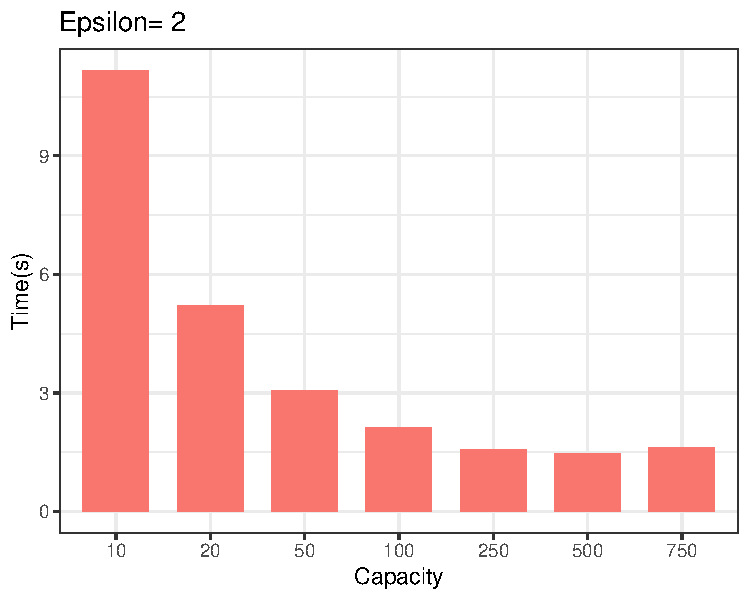
\includegraphics[width=0.45\linewidth]{chapterPFlocks/figures/plots/01_optimal_performance/pflockE2_by_capacity.pdf} & 
         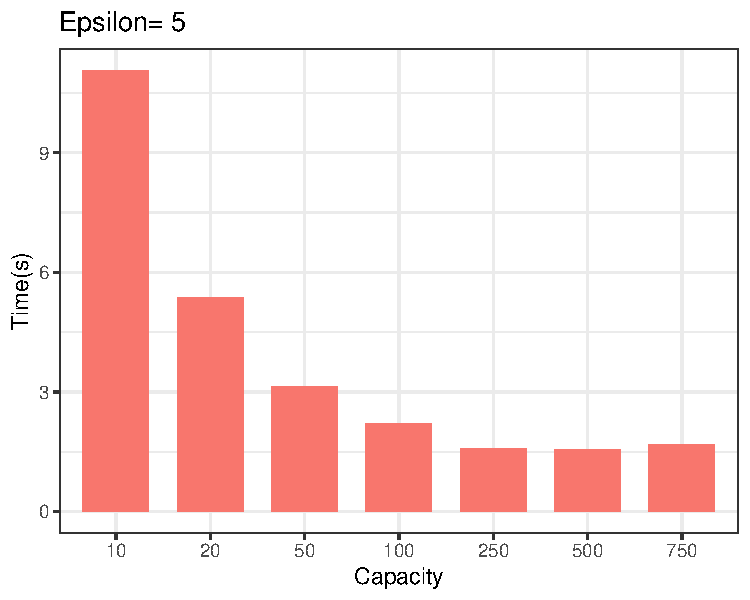
\includegraphics[width=0.45\linewidth]{chapterPFlocks/figures/plots/01_optimal_performance/pflockE5_by_capacity.pdf} \\
         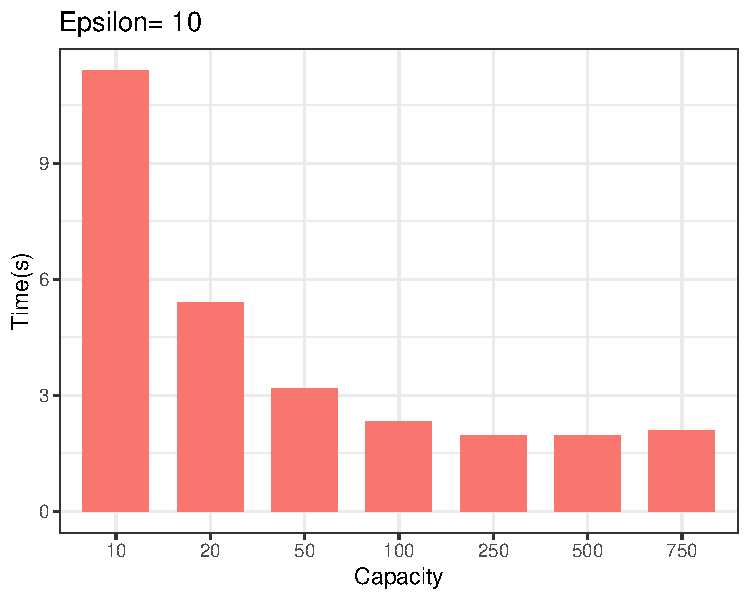
\includegraphics[width=0.45\linewidth]{chapterPFlocks/figures/plots/01_optimal_performance/pflockE10_by_capacity.pdf} &
         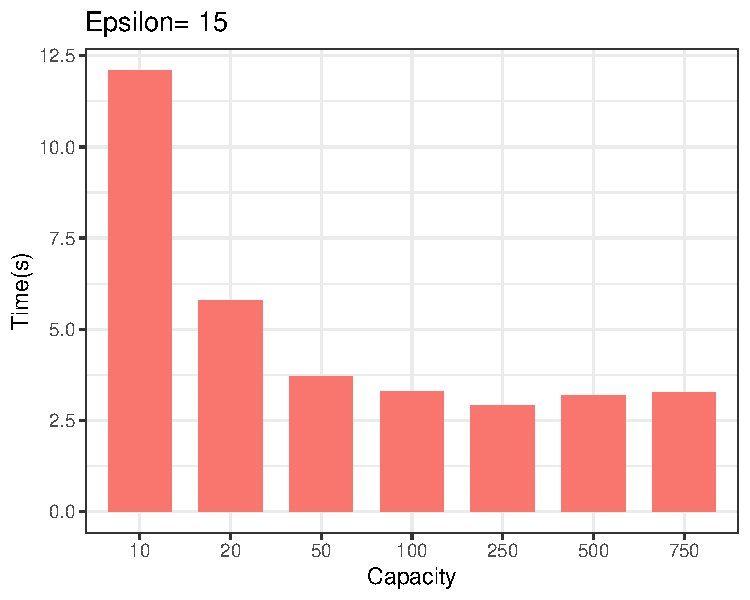
\includegraphics[width=0.45\linewidth]{chapterPFlocks/figures/plots/01_optimal_performance/pflockE15_by_capacity.pdf} \\ 
         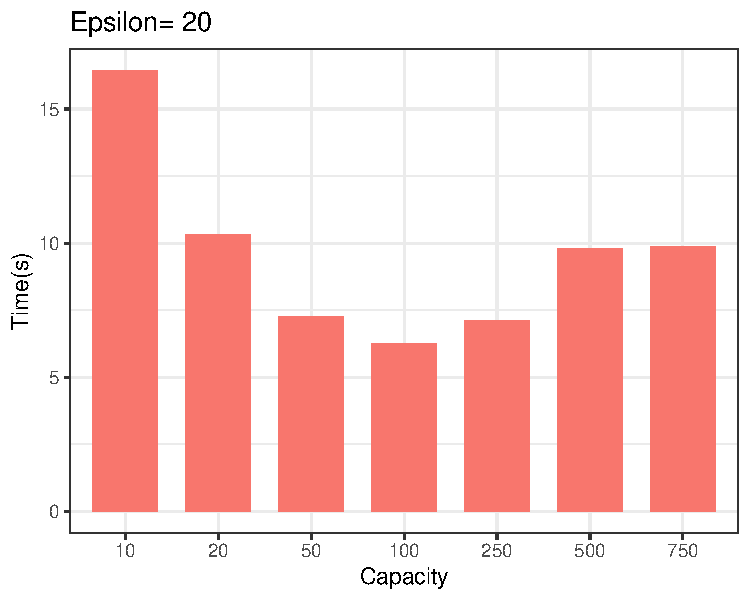
\includegraphics[width=0.45\linewidth]{chapterPFlocks/figures/plots/01_optimal_performance/pflockE20_by_capacity.pdf} & \\
    \end{tabular}
    \caption{Execution time testing different values for Capacity ($c$) and Epsilon  ($\varepsilon$).}\label{fig:optimal_performance}
\end{figure}

After determining the optimal value of $c$ for a given $\varepsilon$, we further analyzed the behavior of BFE and PSI on the most `demanding' partitions, those 
that required the longest time to complete Phase 1. Since the partitions are processed in parallel across different cores, these demanding partitions have the 
greatest impact on the overall performance. By focusing on these partitions, we can better understand potential bottlenecks and further optimize the system's 
efficiency.

\subsection{Analyzing most costly partitions.}
We began by identifying the top 10 partitions that required the most time to execute the BFE algorithm with $\varepsilon = 20$ meters. For these specific 
partitions, we ran both BFE and PSI while varying $\varepsilon$ from 10 to 20 meters. The Phase 1 execution times are shown in Figure 
\ref{fig:top_time_partitions}, where it is evident that PSI consistently outperformed BFE across all values of $\varepsilon$.

\begin{figure}
    \centering
    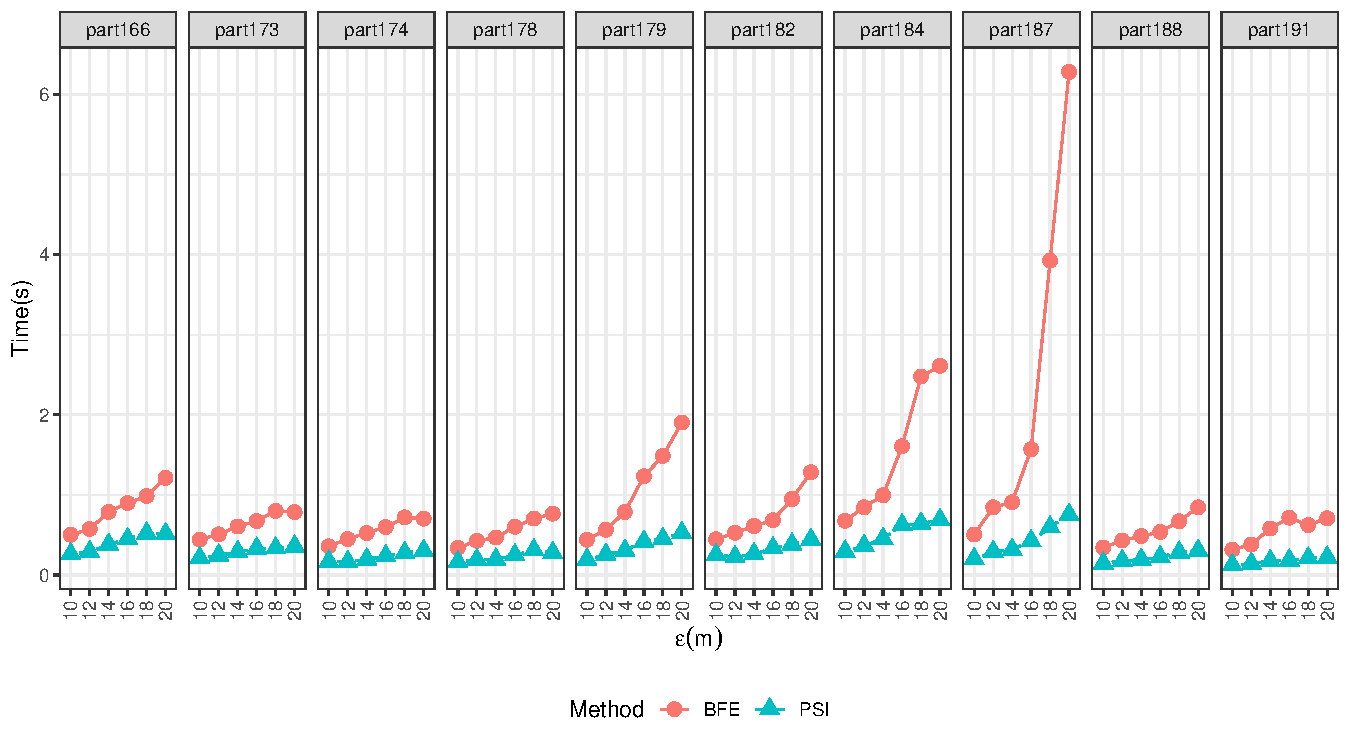
\includegraphics[width=\linewidth]{chapterPFlocks/figures/plots/03_top_time_partitions/top_time_partitions.pdf}
    \caption{Comparing the performance of PSI and BFE for time consuming  partitions.} \label{fig:top_time_partitions}
\end{figure}

We further investigated the reasons behind some partitions taking longer to compute. Figure \ref{fig:pairs_performance} shows the Phase 1 execution times per 
partition while varying $\varepsilon$ from 10m to 20m, with partitions ordered by the number of pairs they contain. One key observation is that as $\varepsilon$ 
increases, the number of pairs also increases, since a larger $\varepsilon$ allows for more maximal disks. For instance, with $\varepsilon = 10m$, the maximum 
number of pairs in a partition is around 1800, whereas for $\varepsilon = 20m$, some partitions contain nearly 4000 pairs.

\begin{figure}
    \centering
    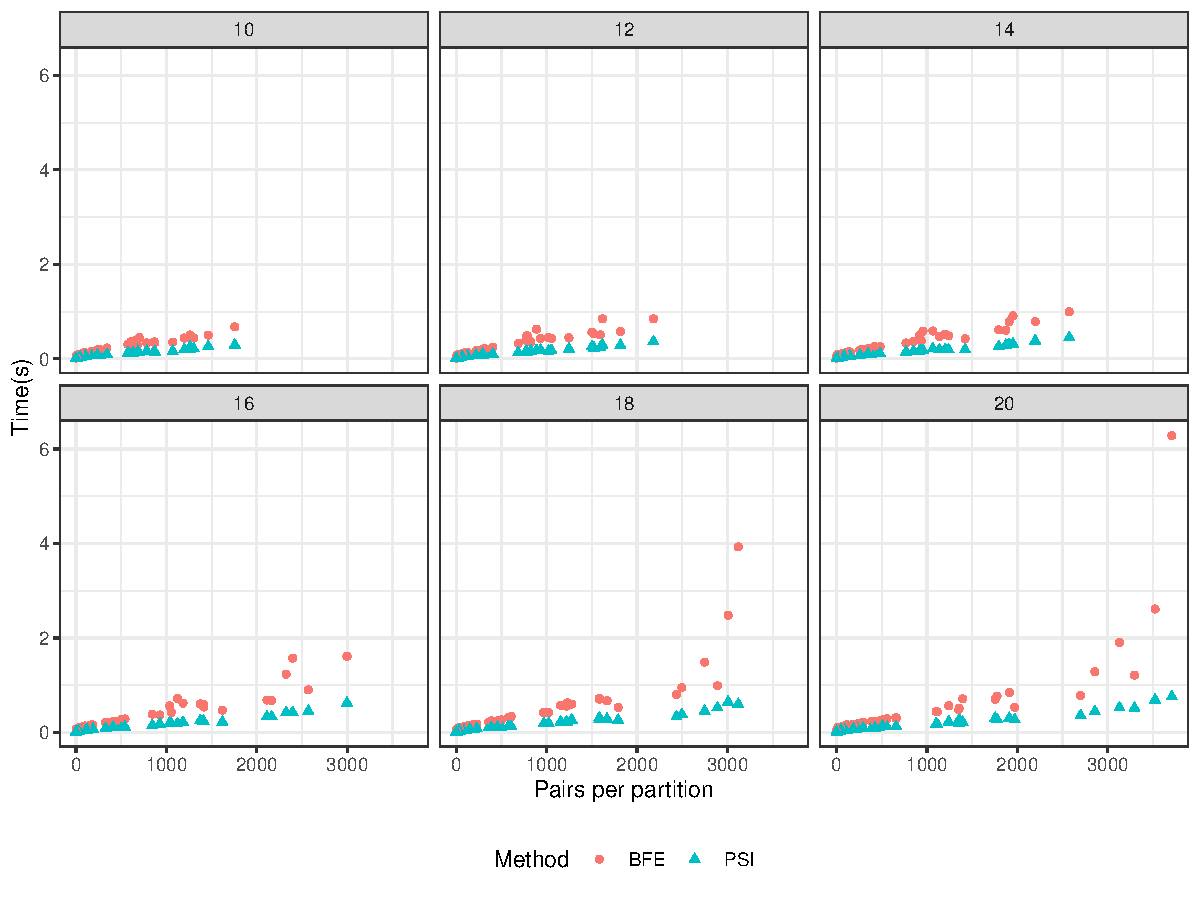
\includegraphics[width=0.85\linewidth]{chapterPFlocks/figures/plots/04_pairs_performance/pairs_performance.pdf}
    \caption{Execution time for pairs/disks finding in the dense partition.}
    \label{fig:pairs_performance}
\end{figure}

Another notable observation is that BFE is more sensitive to the density of pairs within a partition than PSI, a difference that becomes more pronounced at 
higher values of $\varepsilon$ (e.g., 18m or 20m). As mentioned earlier, the flexible bounding boxes used by PSI (illustrated in Figure \ref{fig:square}) more 
effectively isolate the relevant points for computing pairs, whereas BFE relies on a fixed grid cell, which makes it less efficient in denser partitions.

A final observation is that a few partitions take significantly more time than others, particularly those with a higher density of pairs. This is directly 
related to the number of maximal disks that need to be computed and subsequently pruned. For example, the partition that takes the longest time when 
$\varepsilon = 20m$ is the one with the highest number of pairs, which corresponds to partition 187 in Figure \ref{fig:top_time_partitions}.

We further analyzed how Phase 1 processing is distributed within the most demanding partition. Figure \ref{fig:dense_stages}.a (for BFE) and Figure 
\ref{fig:dense_stages}.b (for PSI) display the time taken by each Phase 1 stage (refer to Figure \ref{fig:MF_stages}) for partition 187. The most 
resource-intensive stage in both cases is the final step of filtering the disks, where disks whose points are contained within others are removed—this stage 
identifies the \textit{maximal} disks (labeled as `Maximals' in the figure).

This stage is particularly costly because both BFE and PSI must scan a large set of candidate disks, identifying and removing those that are redundant. As 
$\varepsilon$ increases, this processing becomes even more time-consuming, as the number of pairs and candidate disks grows along with $\varepsilon$.

\begin{figure}
    \centering
    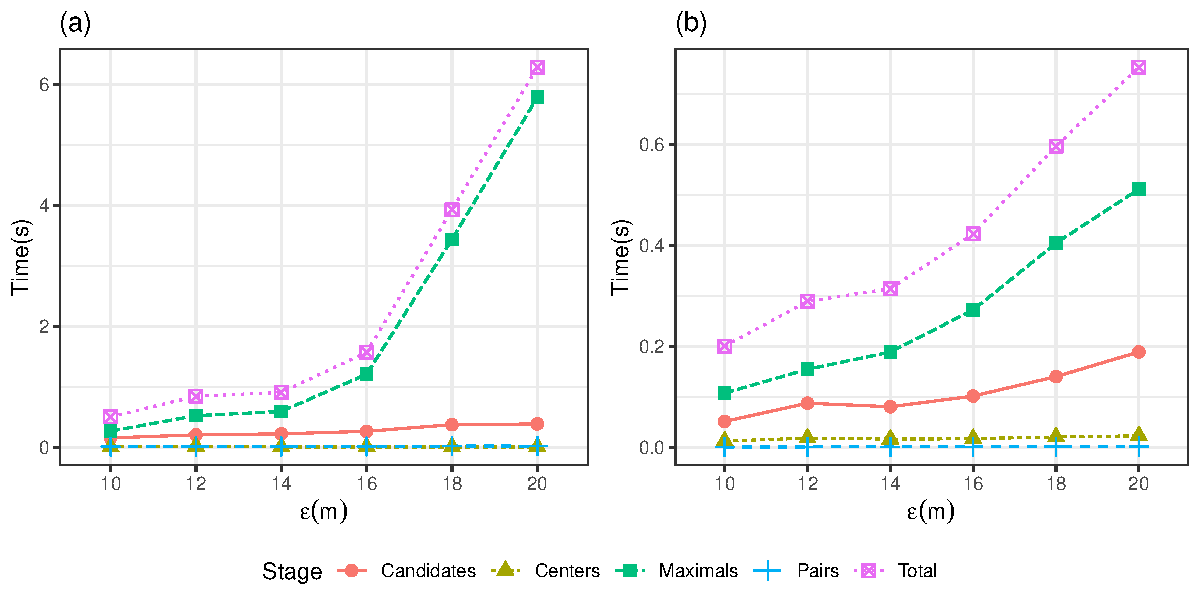
\includegraphics[width=\linewidth]{chapterPFlocks/figures/plots/09_dense_stages/dense.pdf} 
    \caption{Processing time for the stages of Phase 1, in (a) standard BFE and (b) standard  PSI.}\label{fig:dense_stages}
\end{figure}

\subsection{Can we reduce pruning time?}
Dense areas pose challenges for pruning, as they are highly sensitive to increases in the value of $\varepsilon$, leading to an exponential growth in the number 
of pairs. To address this, we explored alternative strategies that could enable more effective grouping of points. It is important to note that density-based 
spatial clustering methods, such as DBSCAN \cite{dbscan}, are not suitable for this problem. In very dense regions, these approaches often produce a single 
large cluster, which does not resolve the issue. Additionally, clustering algorithms do not enforce the strict relationships required for a flock, where all 
points must be within a distance of $\varepsilon$ from each other.

Instead, we explored graph-oriented clustering, focusing on the concept of \textit{maximal cliques}. In an undirected graph, a maximal clique is a subset of 
vertices where each vertex is directly connected to every other vertex in the subset. Additionally, the clique is maximal in the sense that it cannot be 
extended by adding more vertices \cite{tomita_clique_2013, bron_algorithm_1973}.

In this context, the points within a partition can be treated as the vertices of an undirected graph, where edges are created between pairs of points that are 
within a distance of $\varepsilon$. By finding the set of maximal cliques in this graph, we identify subsets of points where each point is connected to all 
others in the subset. This means that all points in the clique are at most $\varepsilon$ apart, and no additional points can be added to the subset.
However, not every maximal clique qualifies as a maximal disk. A maximal clique becomes a maximal disk only if it contains at least $\mu$ points and can be 
enclosed by a disk with a radius of $\frac{\varepsilon}{2}$.

To verify whether a maximal clique qualifies as a maximal disk, we introduce the concept of the \textit{Minimum Bounding Circle} (MBC) \cite{welzl_mbc_1991}. 
Given a set of points in Euclidean space, the MBC is the smallest circle that can enclose all the points. For each maximal clique identified within a partition, 
we can quickly check if all points in the clique fit within an MBC with a diameter of $\varepsilon$. If they do, we can immediately report the set of points and 
their MBC as a maximal disk.  However, cliques that do not satisfy this condition must be evaluated using the traditional method. This involves computing the 
potential disk centers, identifying candidate disks, and pruning them, as outlined in Figure \ref{fig:MF_flowchart}. Figure \ref{app:cmbc_flowchar} illustrates the steps described above.

To evaluate the cliques that do not meet the above condition, we implemented two variants. The first variant, termed \textit{COLLECT}, gathers the points from 
all cliques that are not reported as maximal disks, removes duplicates (since points may appear in multiple cliques), and then applies the traditional pruning 
method to the entire set. In the second variant, \textit{EACH}, we apply the pruning procedure independently for each clique that does not qualify as a maximal 
disk.

Figure \ref{fig:cmbc_variants} compares the performance of these variants against the time taken by BFE (a) and PSI (b) for the same stage. Surprisingly, 
neither variant improves execution time. A closer examination reveals that while identifying the cliques and their MBCs is relatively fast, few cliques actually 
qualify as maximal disks. As a result, the overhead involved in processing the remaining cliques is significant, making the original approach more efficient for 
both BFE and PSI.

\begin{figure}
    \centering
    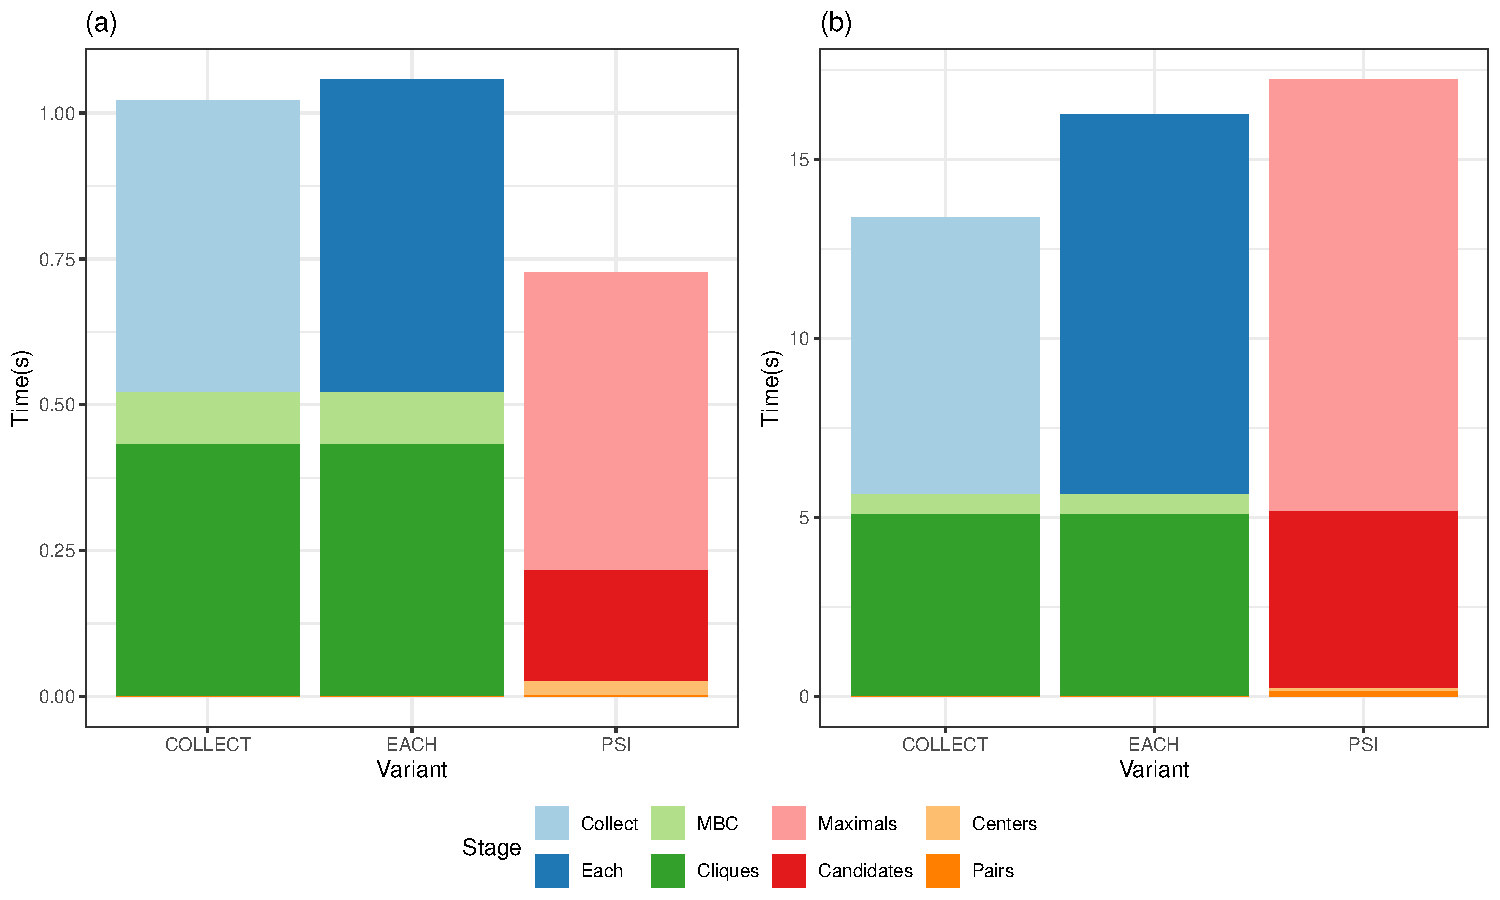
\includegraphics[width=\linewidth] {chapterPFlocks/figures/plots/10_cmbc/cmbc2.pdf}
    \caption{Execution time of the Cliques approach compared to (a) standard BFE and (b) standard PSI.}\label{fig:cmbc_variants}
\end{figure}

\subsection{Relative performance of BFE and PSI Phase 1 using synthetic datasets.}
To further examine the relative performance of the scalable BFE and PSI approaches for Phase 1, we also conducted experiments using a synthetic dataset where we 
could control the values of $c$, $\varepsilon$, and point density. We used a fixed square area of 1000m x 1000m, within which we uniformly distributed 25K, 50K, 
75K, and 100K points.

We experimented with different quadtree capacities ($c$ values of 100, 200, and 300), which resulted in varying numbers of partitions (as shown in Table 
\ref{tab:uniform_ncells}). Both BFE and PSI were tested for phase 1, where maximal disks are identified, using $\varepsilon$ values ranging from 1m to 5m. The 
results are presented in Figure \ref{fig:uniform_performance}.

Overall, PSI demonstrated better performance than BFE, though there were cases (particularly with smaller $\varepsilon$ values) where BFE outperformed PSI. In 
these cases, the smaller $\varepsilon$ generates fewer pairs, and the additional ordering step required by PSI becomes an overhead. However, in the subsequent 
experiments focusing on temporal joins (phase 2, flock creation), we concentrate on the scalable performance of PSI.

\begin{table}
    \centering
    \caption{Number of partitions by capacity and number of points in synthetic uniform datasets.}
    \label{tab:uniform_ncells}
    \begin{tabular}{c|cccc}
              & 25K & 50K  & 75K  & 100K \\
        \hline
        c=100 & 544 & 1024 & 1024 & 2185 \\
        c=200 & 256 & 514  & 1024 & 1024 \\
        c=300 & 256 & 514  & 481  & 1024 \\
    \end{tabular}
\end{table}

\begin{figure}
    \centering
    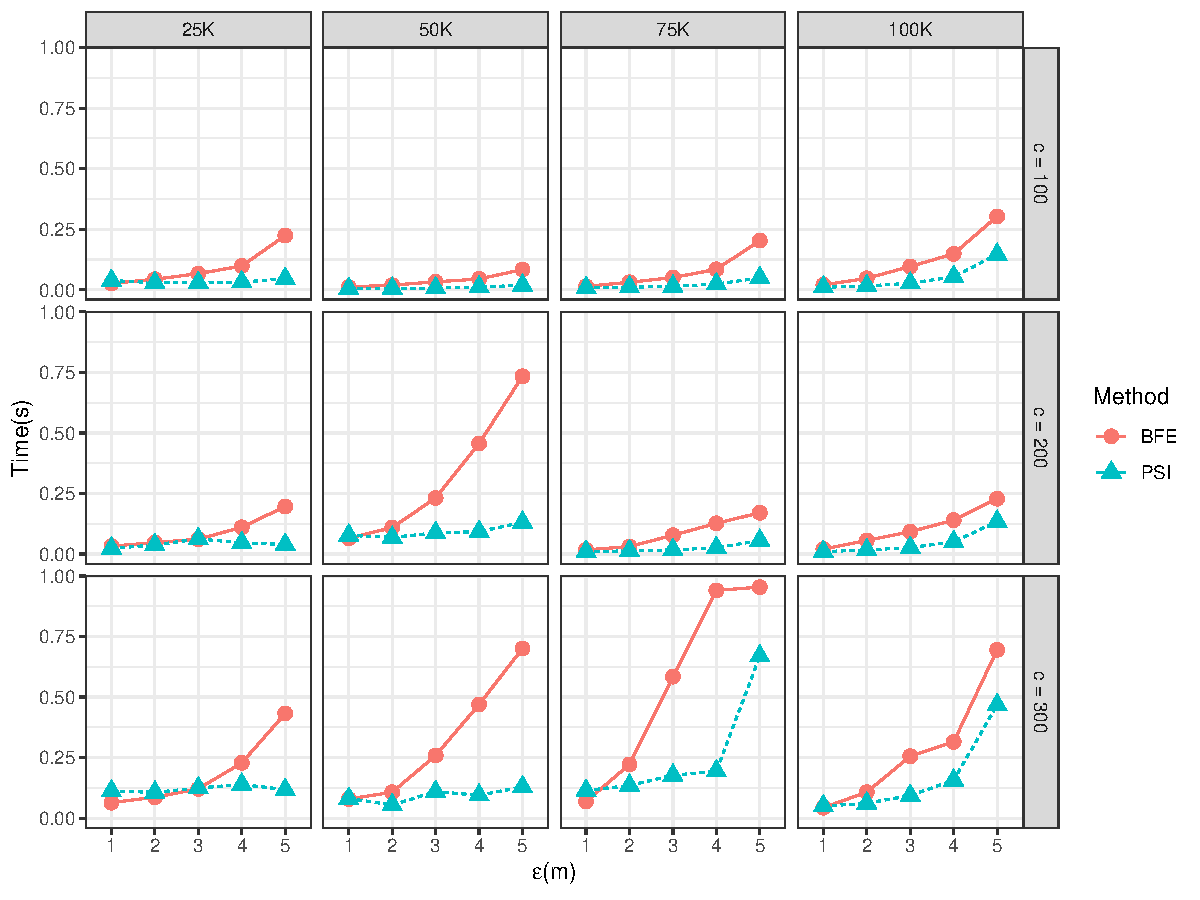
\includegraphics[width=\linewidth]{chapterPFlocks/figures/plots/05_uniform_performance/uniform_performance.pdf}
    \caption{Performance in an uniform dataset analysing density and capacity with diverse values for epsilon.}\label{fig:uniform_performance}
\end{figure}

\subsection{Evaluation of Phase 2: Temporal join.}
Phase 2 focuses on joining maximal disks across time instants to form flocks. In Section \ref{sec:temporal_join}, we discussed four alternatives: Master, 
By-Level, LCA, and Cube-based. For these experiments, we used the scalable PSI approach due to its robust performance.
First, we compared the Master and By-Level alternatives while varying $\varepsilon$ from 20m to 40m using the Berlin10K dataset (see Figure 
\ref{fig:step_performance}). For the By-Level approach, we tested different step values ranging from 1 to 6. The Master approach proved to be the slowest, due 
to the overhead of sending all CPFs to the root node. The performance of the By-Level approach depends on the step size. A smaller step value (e.g., step 1) 
introduces overhead because CPFs may need to be evaluated at more intermediate nodes before completion. On the other hand, a larger step value reduces 
parallelism by sending more CPFs to intermediate nodes. Based on these experiments, we determined that Step=3 offers the best balance.

We also evaluated the optimal value for the \textit{interval} parameter in the Cube-based approach. Using the LA25K dataset with $\varepsilon=30m$, we tested 
various interval values, ranging from 2 to 12 time instants. This dataset contains 30 time instants in total. The results, shown in Figure 
\ref{fig:interval_performance}, illustrate the trade-offs involved. Lower interval values result in higher parallelism, as more cubes can be processed 
independently. However, this also increases the number of cube crossings for CPFs that need to be checked, which adds to the execution time. Conversely, larger 
interval values reduce parallelism but also decrease the number of CPF crossings. Based on these findings, we selected $interval=6$ as the optimal value for the 
Cube-based approach.

\begin{figure}
    \centering
    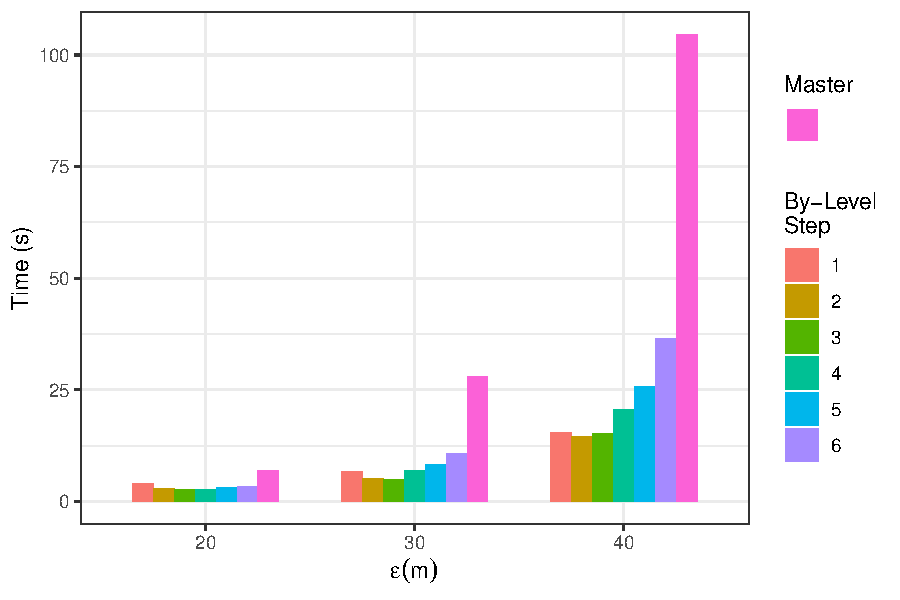
\includegraphics[width=0.8\linewidth]{chapterPFlocks/figures/plots/06_step_performance/step_performance.pdf}
    \caption{Root and step alternative for temporal join using the Berlin dataset.}\label{fig:step_performance}
\end{figure}

\begin{figure}
    \centering
    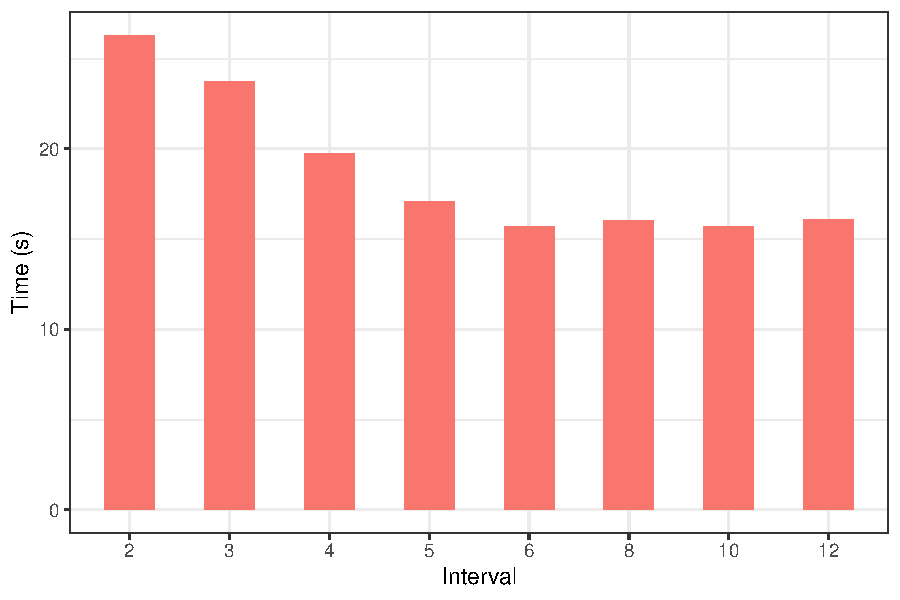
\includegraphics[width=0.8\linewidth]{chapterPFlocks/figures/plots/07_interval_performance/interval-performance.pdf}
    \caption{Interval optimization for the Cube-based alternative for temporal join using the LA25K dataset.}\label{fig:interval_performance}
\end{figure}

Finally, we compared the optimized versions of the By-Level and Cube-based approaches with the Master and LCA methods. Figure \ref{fig:la25k_e_bfe_psi} shows 
the results, including the sequential PSI algorithm as a reference. This experiment was conducted using the LA25K dataset with $\varepsilon$ values ranging from 
5m to 30m. Clearly, all parallel approaches offer significant improvements over the sequential PSI.

To further analyze the relative performance of the scalable approaches, Figure \ref{fig:la25k_e} focuses on the parallel algorithms for the same experiment. 
Interestingly, for very small $\varepsilon$ values, the Master approach performs best —primarily because the limited number of flocks makes sending the CPFs to 
a single node fast and efficient. However, as $\varepsilon$ increases, the Cube-based approach becomes the most effective, leveraging greater parallelism. 
By-Level also improves over the Master approach as $\varepsilon$ grows, as explained in Figure \ref{fig:step_performance}. Similarly, for larger $\varepsilon$ 
values, the LCA approach outperforms By-Level because it more quickly identifies the node that can complete the CPF operations.

We repeated the same experiment with the LA50K dataset, varying $\varepsilon$ from 4m to 20m. The results, shown in Figure \ref{fig:la50k_e}, once again 
demonstrate that the Cube-based approach offers the best performance as $\varepsilon$ increases.

\begin{figure}
    \centering
    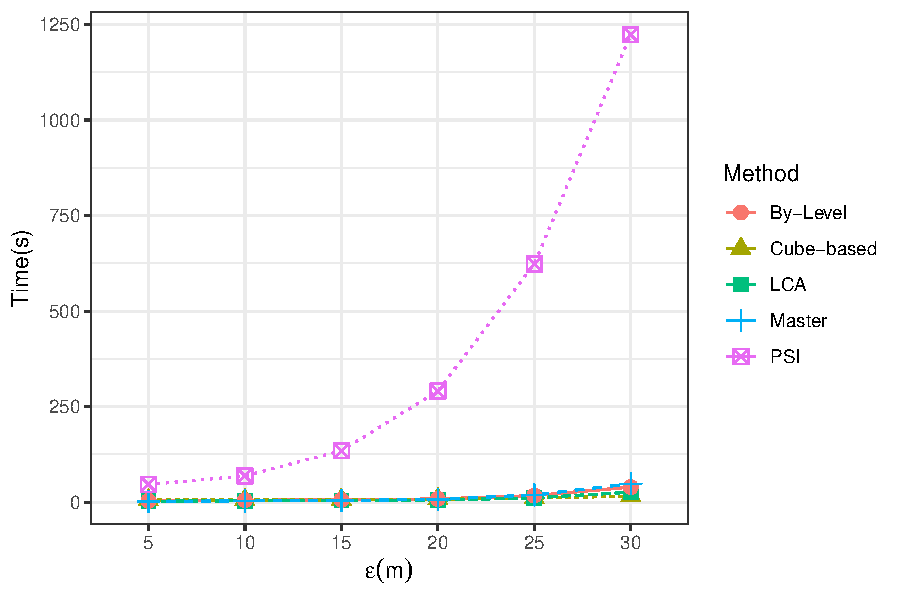
\includegraphics[width=0.75\linewidth]{chapterPFlocks/figures/plots/08_sequential_parallel/la25k_e_bfe_psi.pdf}
    \caption{Performance comparing parallel and sequential alternatives in the LA25K dataset.}\label{fig:la25k_e_bfe_psi}
\end{figure}

\begin{figure}
    \centering
    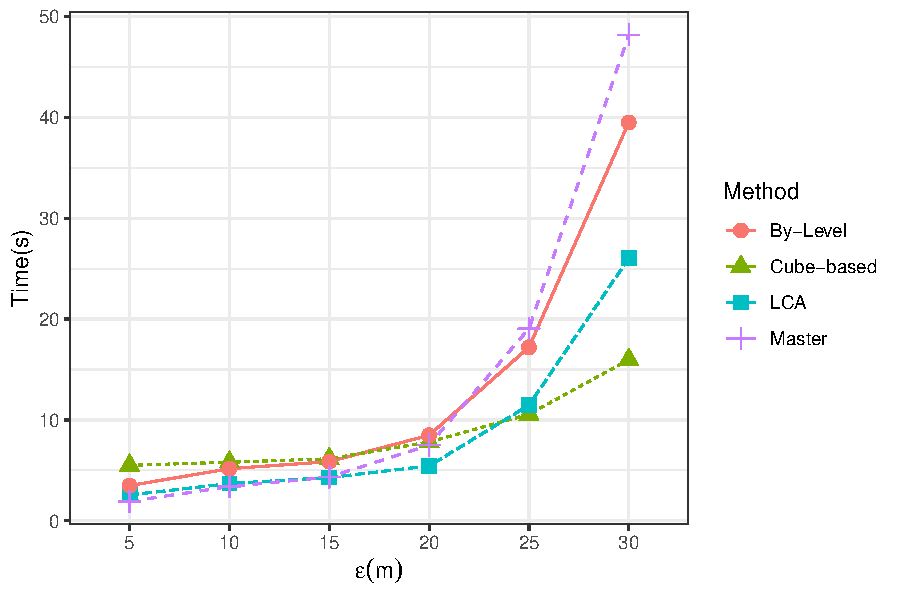
\includegraphics[width=0.75\linewidth]{chapterPFlocks/figures/plots/08_sequential_parallel/la25k_e.pdf}
    \caption{Performance of the 4 parallel alternatives in the LA25K dataset.}\label{fig:la25k_e}
\end{figure}

\begin{figure}
    \centering
    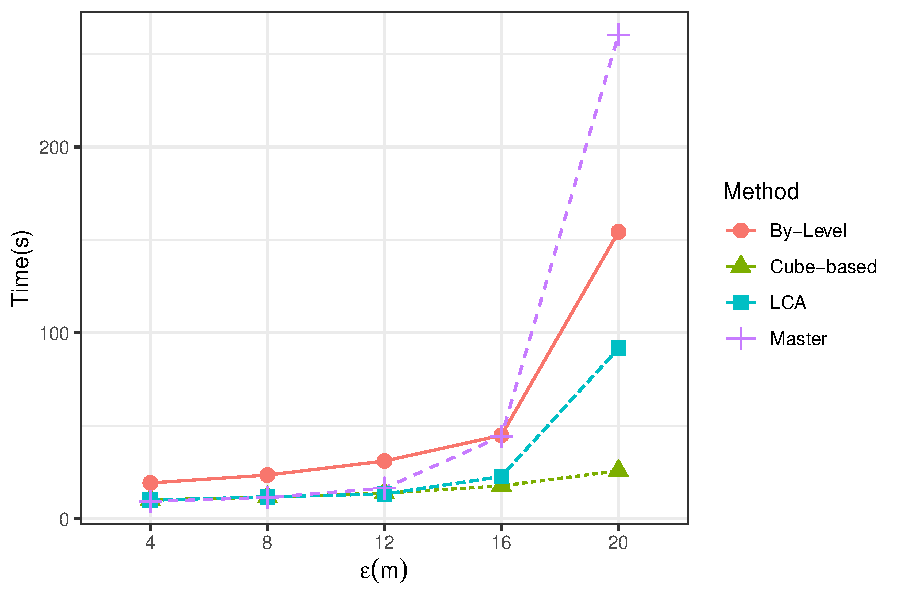
\includegraphics[width=0.75\linewidth]{chapterPFlocks/figures/plots/08_sequential_parallel/la50k_e.pdf}
    \caption{Performance of the 4 parallel alternatives in the LA50K dataset.}\label{fig:la50k_e}
\end{figure}
